\section*{Exercice 1}
\begin{wrapfigure}{r}{0.5\textwidth}
    \begin{center}
    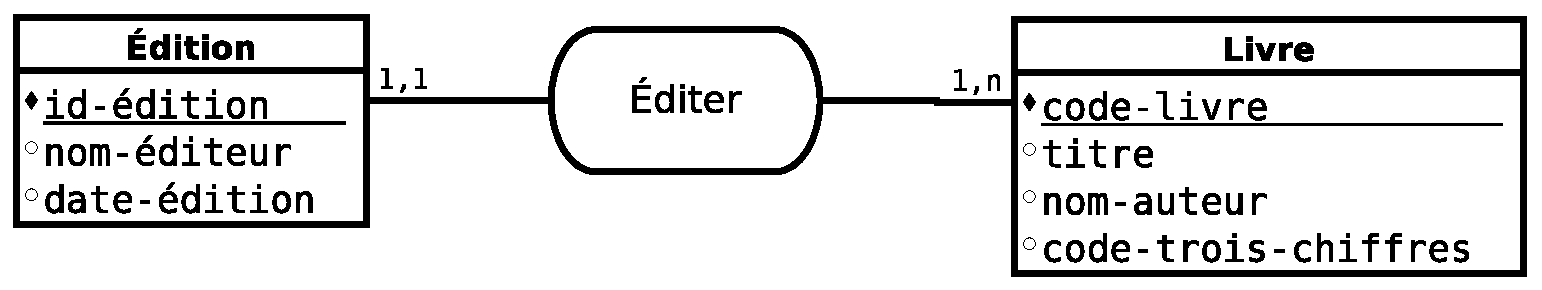
\includegraphics[width=0.4\textwidth]{images/partie_mcd.eps} 
    \caption{\label{mcd} Partie du MCD}
    \end{center}
\end{wrapfigure}
Une première analyse du système d'information de la Bibliothèque Universitaire (BU) a révélé des erreurs dans sa conception actuelle. Expliquez ce qui ne convient pas ici et donnez une version corrigée sachant que : 
\begin{itemize}
    \item Le code d'un livre est composé du code de la bibliothèque où il se trouve, du code de son auteur principal, de son année d'édition, et d'un numéro sur trois chiffres 
    \item le numéro sur trois chiffres du code d'un livre est défini lors de l'achat de celui-ci par la BU, il correspond au nombre de livres du même auteur détenus par la BU, mais on veut pouvroir changer cette règle de numérotation dans le futur si besoin
\end{itemize}

\section*{Exercice 2}
Lors de son inscription, chaque étudiant doit choisir une bibliothèque dite de "référence" mais peut emprunter un livre dans toutes les bibliothèques de la BU\@. La BU veut s'assurer qu'un livre est emprunté le plus souvent par des étudiants ayant choisit la bibliothèque où il se trouve en tant que bibliothèque de référence. 
La BU de l'Exercice~1, vous demande de continuer à modéliser son système d'information avec les contraintes suivantes : 
\begin{itemize}
    \item Le code d'un livre est composé du code de la bibliothèque où il se trouve, du code de son auteur principal, de son année d'édition, et d'un numéro sur trois chiffres 
    \item le numéro sur trois chiffres du code d'un livre est défini lors de l'achat de celui-ci par la BU, il correspond au nombre de livres du même auteur détenus par la BU, mais on veut pouvroir changer cette règle de numérotation dans le futur si besoin
    \item Chaque année, la BU souhaite évaluer le nombre d'emprunts d'un livre 
    \item Si un livre se trouvant dans une bibliothèque est emprunté plus souvent par des étudiants ayant choisit une autre bibliothèque de référence, le livre est changé de bibliothèque
\end{itemize}

\subsubsection*{documents et données jugés utiles}
\begin{itemize}
    \item Carte d'étudiant (numéro de carte, nom de l'étudiant, bibliothèque de référence)
    \item Livre (code livre, titre, noms des auteurs, nom de l'éditeur)
\end{itemize}

\subsubsection*{notes}
\begin{itemize}
    \item Le résultat de l'Exercice~1 fait partie de la réponse.
\end{itemize}
